% !Mode:: "TeX:UTF-8"
\chapter{Introduction}

TODO: Introduction

JPEG is widley used in image compression applications. It was introduced in 1992 \cite{wallace_jpeg_1992}. Algorithm consists of several steps. Chroma subsampling is a process of transformations from RGB format to YCbCr. YCbCr is a special format of storing image data not in Red, Green and Blue channels, but in Y, Cb and Cr channels. Y is the brightness channel of an image, Cb is the blue difference relative to the green color, Cr is the red difference relative to the green channel. After that it is already possible to reduce size by rescaling Cb and Cr channels by four. By doing so, the space is reduced by 1.5.

Compression of each channel is an performed in parallel. Image is partitioned into blocks 8x8 pixels. Each block is processed independently. Block values are centered at 0, so the values are in range (-127, 127). Then Discrete Cosine Transform (DCT) is being applied.

TODO: describe an algorithm of DCT.



Nowadays there are many existing image compression approaches. We can divide such algorithms in two groups: lossy (such as JPEG. Mainly such algorithms use Discrete Cosine Transform) and lossless (such as DEFLATE. Mainly such algorithms use similar to Huffman Encoding methods). Both has beed developed for decades already. It is important to mention that image containers (such as JPEG, PNG, GIF etc.) use information compression algorithms \textit{only as a part} of their architecture. Usually lossy and lossless compression methods are combined to achieve higher performance.

Famous JPEG format, for example, has following steps, and only last three are about compression.

\begin{enumerate}
    \item Transformation from RGB to YCbCr (Chroma subsampling).
    \item Quantization. Lossy.
    \item Discrete Cosine Transform. Lossless.
    \item Run-length encoding. Lossless.
    \item Huffman encoding. Lossless.
\end{enumerate}

There is a certain trend to apply a power of neural networks in compression domain, extending a group of lossy algorithms. First approaches were \cite{Balle_Laparra_Simoncelli_2017}, \cite{Theis_Shi_Cunningham_Huszar_2017}, \cite{Toderici_Vincent_Johnston_Hwang_Minnen_Shor_Covell_2017}, where authors proved that we can use one neural network to generate a compressed representation of an image and another neural network to restore initial image from its representation generated by first network. Now such networks are also being used to solve an image and video upscale tasks.

For now a general approach is to encode an image to compressed representation using convolutional neural network and take the convolutional features from one of the top layers of network. In this work we are going to use a slightly different architecture. There were many publications connected to graph convolution in recent years. Early publications introduced a graph convolution, later the main approaches had been formed. It is important to mention that even though the first application were obviously connected to graph classification and graph clustering \cite{Kipf_Welling_2017}, \cite{Defferrard_Bresson_Vandergheynst_2017}, \cite{Fey_Lenssen_Weichert_Muller_2018}, \cite{Hamilton_Ying_Leskovec_2017}, \cite{Hamilton_Ying_Leskovec_2018}, \cite{Monti_Boscaini_Masci_Rodolà_Svoboda_Bronstein_2017}, \cite{Monti_Otness_Bronstein_2018}, \cite{Velicković_Cucurull_Casanova_Romero_Liò_Bengio_2017}, in recent years application domain has been extended to action recognition \cite{Cheng_Zhang_He_Chen_Cheng_Lu_2020}, supply-demand prediction \cite{Jin_Xia_Liu_Murata_Kim_2021}, time series prediction \cite{Cheng_Zhang_He_Chen_Cheng_Lu_2020}, traffic and wind prediction \cite{Cui_Henrickson_Ke_Wang_2020}, \cite{Stańczyk_Mehrkanoon_2021} and many others.

In this work we are going to apply graph convolution algorithms to generate a representation of an image that takes less space and can be transported or stored more effectively. The core of this framework is scene graph representation of an image. It worth to mention that the algorithm we are working on is lossy.

The contribution of this work can be considered from two major perspective. The first is that this work is going to be the first try to use scene graph as a compressed representation of an image. From the second perspective we are going to use a general autoencoder architecture with meaningful graph structure as a representation.

\chapter{Objective}

The first question is how do we memorize some image or visual scene in our life. We do not operate in terms of pixels or object coordinates. More likely we use something like scheme, which describes the most important parts of an image as it shown on \ref{image_and_scene_graph}.

\begin{figure}[!h]
    \centering
    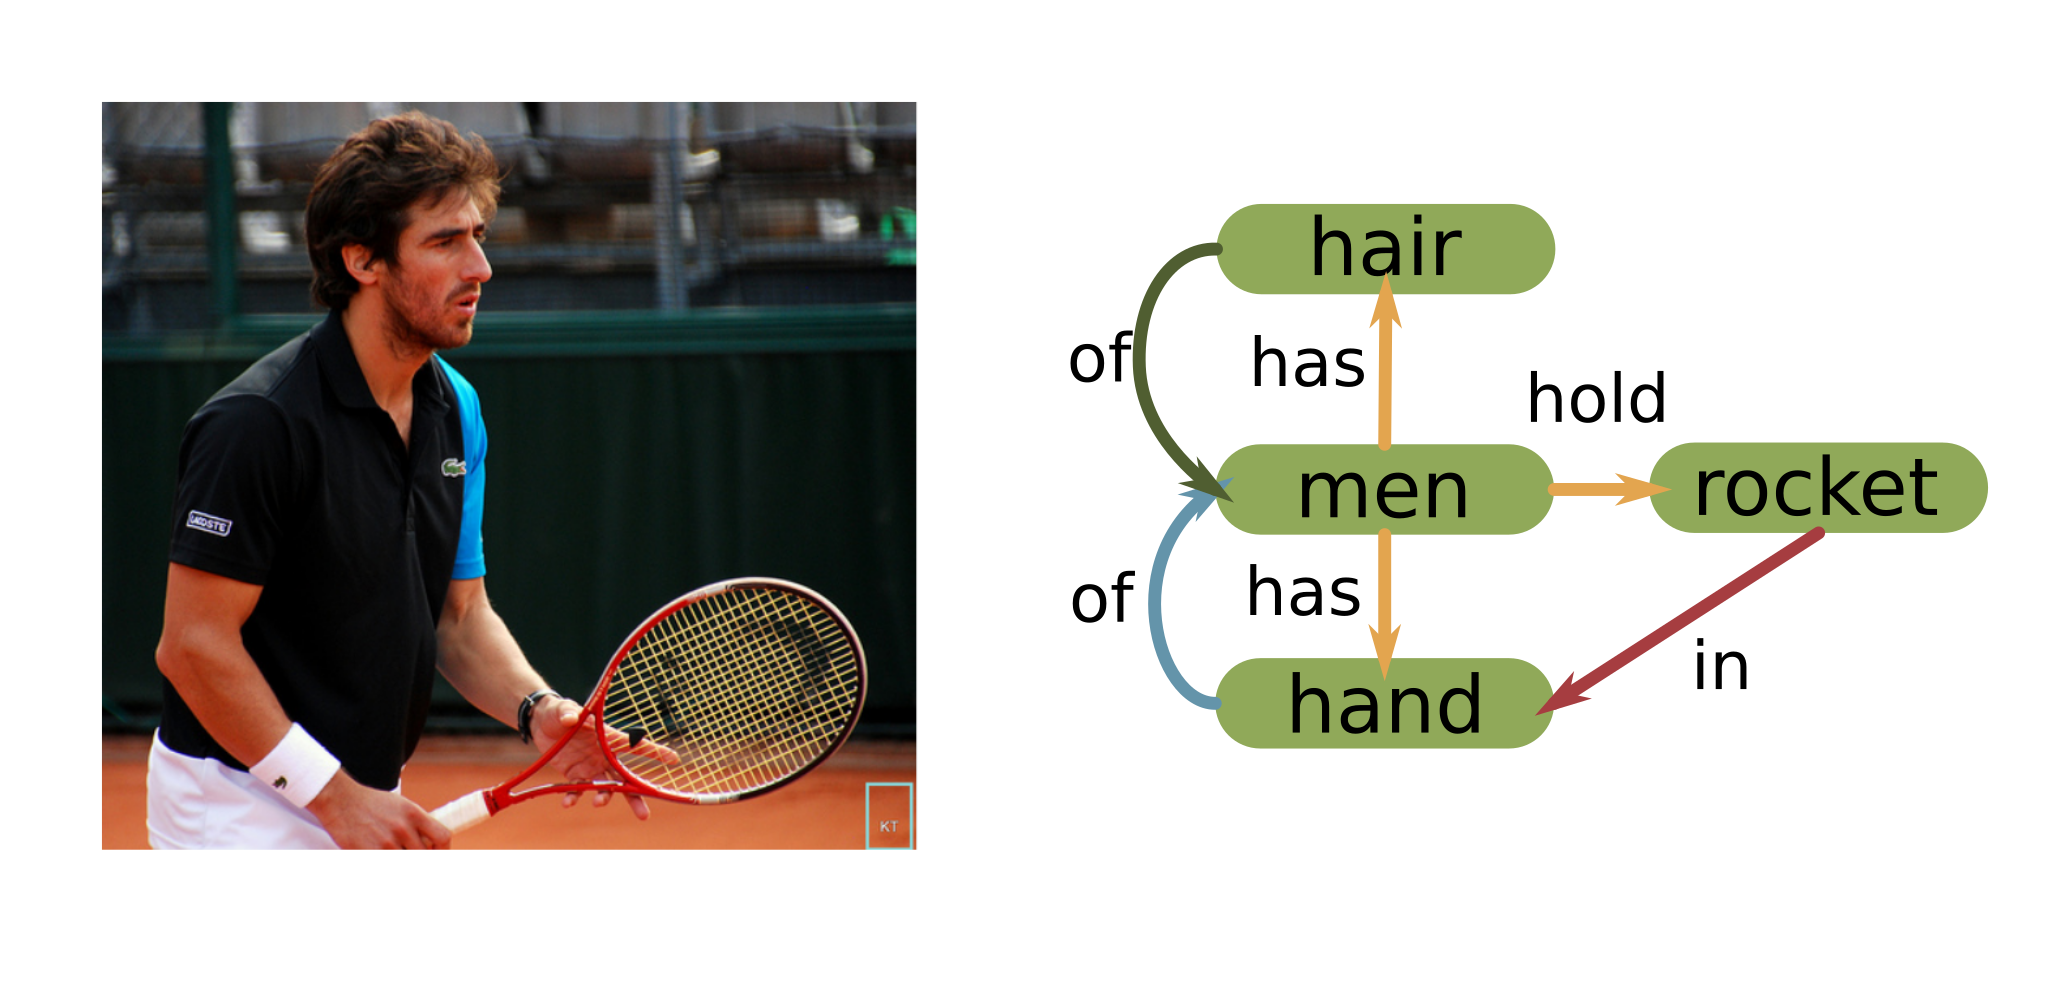
\includegraphics[width=\textwidth]{figure/image-and-scene-graph.png}
    \caption{Image and scene graph associated with it.}
    \label{image_and_scene_graph}
\end{figure}

The scene graph represented on the figure above is simplified, real graph can also have node attributes different from just an object label, for example in case of hair we can also attach an attribute "brown" and "curly".

There are algorithms that can extract a scene graph from an image. There were some approaches to generate image based on scene graph. So the idea is quite obvious: let us combine those two algorithms to build a compression algorithm prototype. From general point of view we can see such algorithm as an autoencoder with Scene Graph Generation network as encoder and Scene Graph to Image network as decoder.

\chapter{Niches}

Potentially this work can improve existing image compression algorithms. We think that the size of scene graph is way more small than size of JPEG. Such an algorithm can be used in different scenarios. Mainly we can use it in traditional use cases for lossy compression such as using it in image format as it is or in more advance sense, to extend existing formats. For example we can extend existing DCT (Discrete Cosine Transform) or DWT (Discrete Wavelet Transform). We selected two possible use cases to apply the compression algorithm we are developing:

\begin{enumerate}
    \item Limited space on machine with high computational power. It can be a big server with powerful CPU. In recent days there are some movements in quantum computing sphere, so it can be a very powerful machine with quantum CPU etc.
    \item Huge images needed to be transmitted through a network with limited speed. In case of a limited performance of a network we can compress and restore images using application, we are working on.
\end{enumerate}

Few years ago already a reasonable performance has been achieved using an encoder-decoder architecture \cite{Theis_Shi_Cunningham_Huszar_2017}. We suppose, that our approach can boost performance both in sense of visual appearance and sense of compressed image size.

\chapter{Methodology}

The main contribution of this work is applying a graph convolution in image compression domain. But let us first define what graph convolution actually is. Convolution is already widely used in image and video processing, and mainly convolutional neural networks (CNNs) consist of stacked layers of such convolutions \cite{Krizhevsky_Sutskever_Hinton_2017}, \cite{Simonyan_Zisserman_2015}. In many architectures authors use learnable \textit{filters} to get representation of the next layer of a network. Convolutional architecture is not new, but it has been widely spread in the last decade because of enormous computation power growth. The main idea of Graph Convolutional Networks is originated from CNNs and generalizes CNN approach from fixed grid structure to arbitrary grid-like graph structure.

In case of this work we can consider scene graph as such structure \ref{application-general-pipeline} with objects obtained from Object Detection step represented as nodes of this graph, attributes of such nodes can be extracted attributes of an object (here we can simply use output of the last convolutional layer of this object region). Applying graph convolution on such graph we can obtain relationships information, and talking about graphs we can treat such relationships as an edges. So, after this step we obtain so called \textit{Scene Graph}, which represents a meaningful information about image. We can also design a generation model and then restore image from such representation. The image obtained from the last step will not be identical, and the purpose of this work is to design such an algorithm that will produce similar enough image.

\begin{figure}
    \centering
    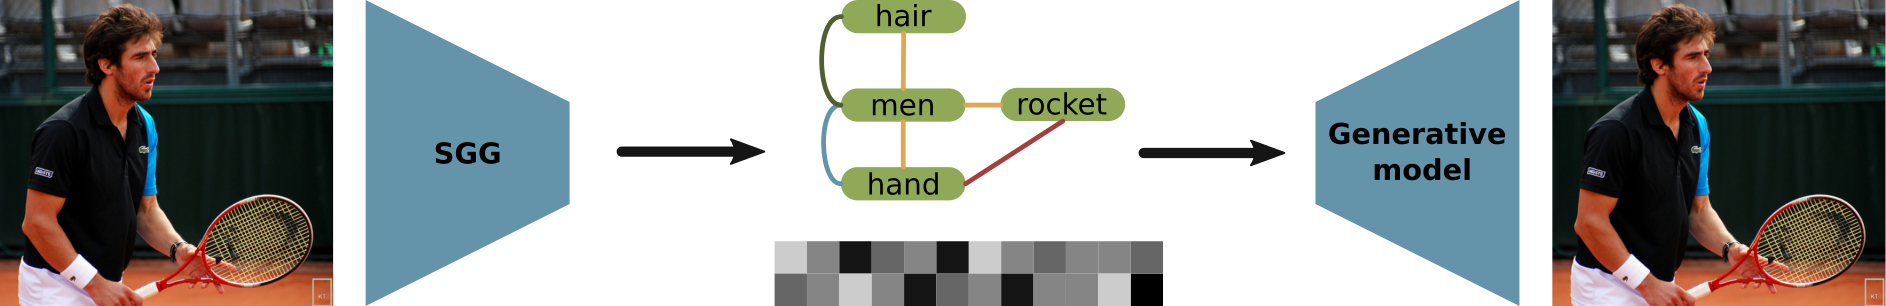
\includegraphics[width=\textwidth]{figure/application-general-pipeline.png}
    \caption{Application general pipeline. First scene graph and convolution features are obtained. Then this can be treated as a compressed representation of initial image. It can be sent through network or being stored on machine. When the original image is needed we can feed this representation to generative model to obtain initial image.}
    \label{application-general-pipeline}
\end{figure}

Application general pipeline can be divided on three steps:

\begin{enumerate}
    \item Scene Graph generation. Having an image as an input on this step we need to generate a scene graph of this image. Here is an example of an image and its scene graph \ref{image-and-scene-graph}
    \item Image generation based on scene graph. Having a scene graph on this step we need to generate (or restore) image.
\end{enumerate}

\begin{figure}[!h]
    \centering
    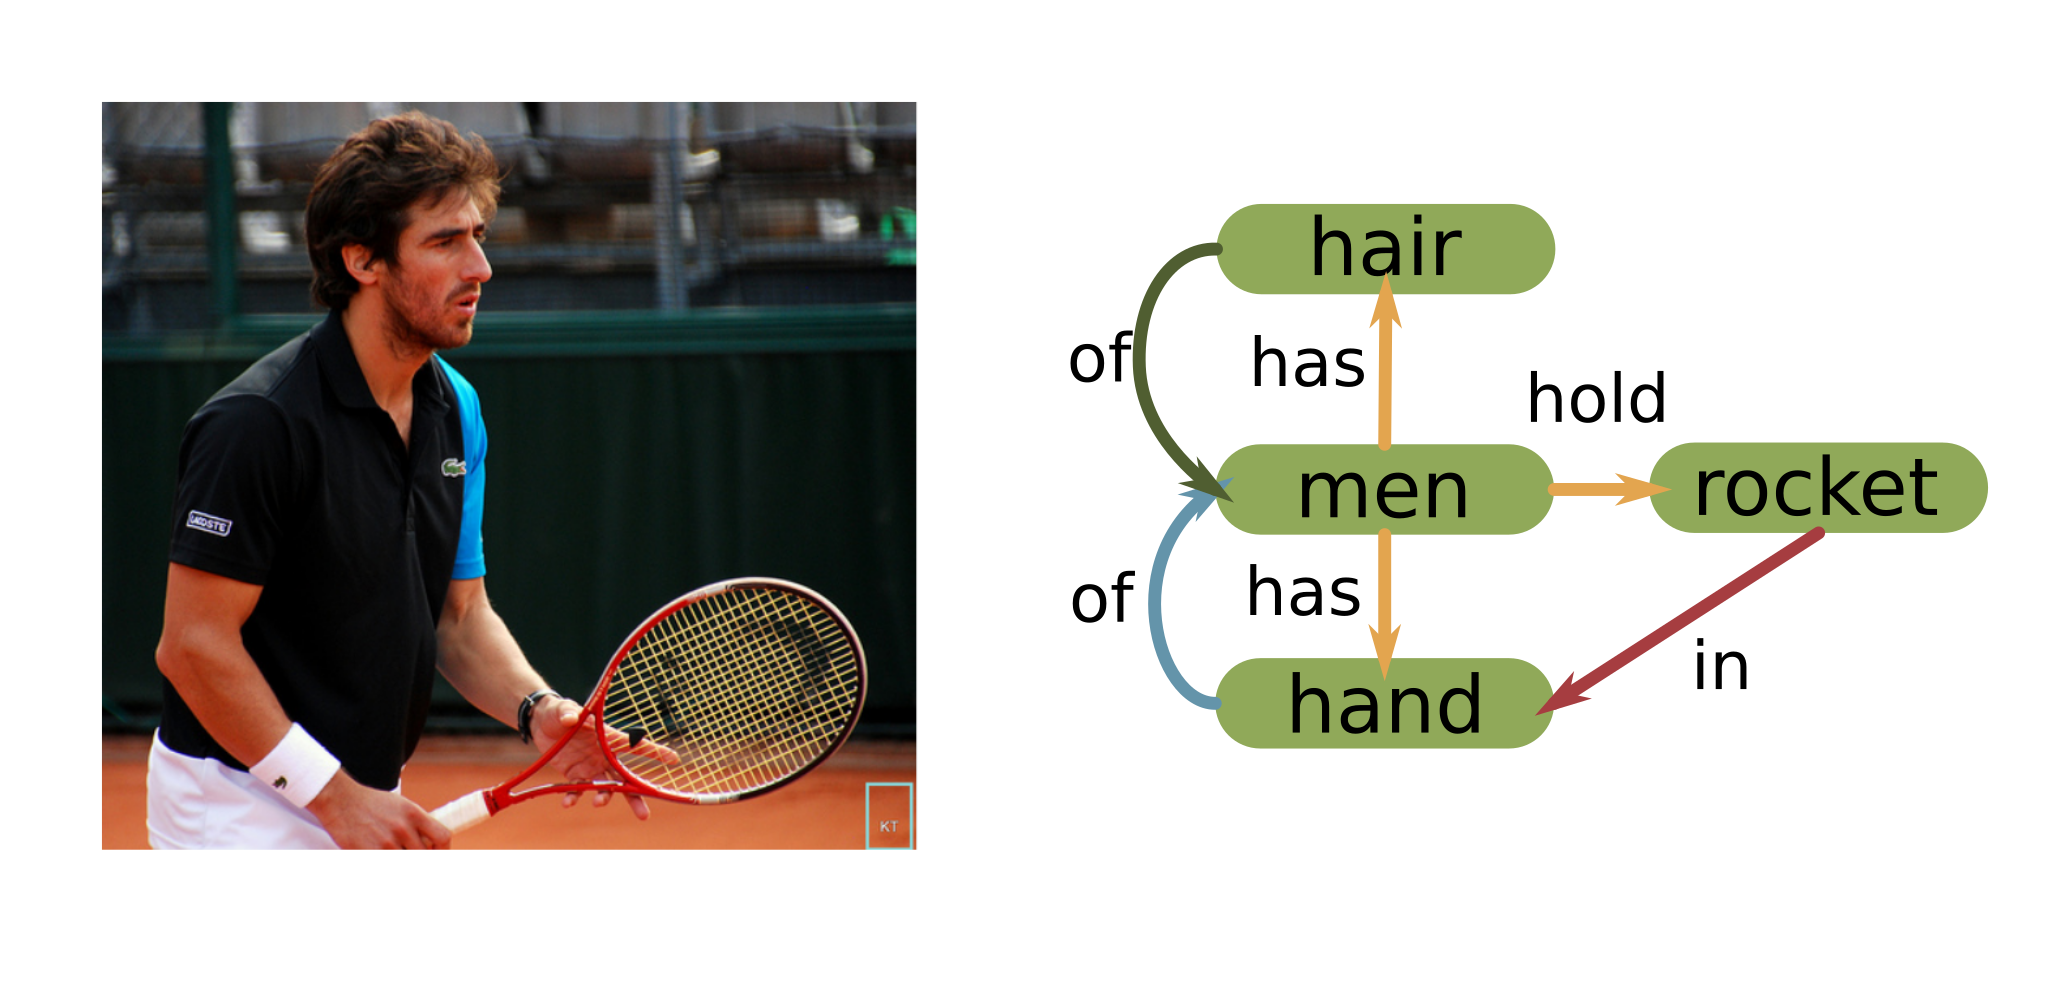
\includegraphics[width=\textwidth]{figure/image-and-scene-graph.png}
    \caption{Image and its scene graph}
    \label{image-and-scene-graph}
\end{figure}

The first thing we want to do is object detection. We need labeled objects regions, that were detected from image. Now there are many various object algorithms, they are already quite advanced and we can simply choose one of them and use as it is. There are a couple of possible choices: FastRCNN, Object detection with transformers, YOLOv5 etc.

After object detection algorithm applied we will have a list of regions and the classes for each region \ref{objects-detected}, we will also need a convolutional features for each region (it will be just a small vector of values obtained from top convolutional layer). Having all the listed we have enough information to build a scene graph and restore image when it is needed. mMore concrete we can use information about detected object regions as a hint to restore original image.

\begin{figure}[!h]
    \centering
    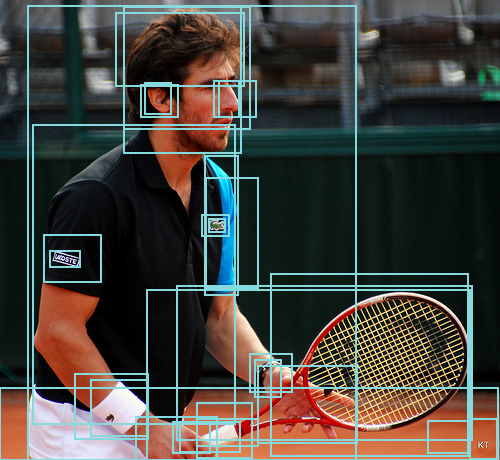
\includegraphics[width=\textwidth]{figure/object-detected.png}
    \caption{Example of detected objects using FastRCNN}
    \label{objects-detected}
\end{figure}

Next we start building a scene graph. Scene graph can be built using different approaches, but we decided to use an approach with graph convolutional networks, since it shows a nice performance and, probably, graph convolution has a bit of potential now. There are still many publications in this sphere.

To be more concrete, let us introduce a simple graph convolution pipeline. Let graph $G$ have a node set $v\in V$ and edge set $e\in E$. Such graph can be represented as square adjacency matrix $A\in \mathbb{Z}^{N\times N}$, where $A_{ij}=0$ if nodes $v_i$ and $v_j$ are not connected. Otherwise, if nodes are connected, then $A_{ij}$ is equal to the weight of the edge $e_{ij}$ between nodes $v_i$ and $v_j$.

Conceptually, convolution operation in CNNs is used to \textit{aggregate} data from fixed neighborhood. For example in pictures it is neighboring pixels (first-order neighbors in case of $3\times 3$ filter, first-order and second-order neighbors in case of $5\times 5$ filter etc.). After that an activation function is being applied. This is the simplest pipeline, and, of course, there is quite a bit of optional layers such as pooling or residual \cite{He_Zhang_Ren_Sun_2015}.

Basically learning on graphs consists of several steps:

\begin{enumerate}
    \item \textbf{Aggregate}. On this step we gather information from neighboring nodes and summarize it.
    \item \textbf{Combine}. On this step we combine aggregated information and own information of current node.
\end{enumerate}

Most of existing frameworks can be expressed in a way presented in \ref{eq:4}. So, both aggregate and combine steps are customizable, and essentially in those steps the main differences between architectures happens.

\begin{equation}
    \label{eq:4}
    h_i^{(l)}=COMBINE(h_i^{(l-1)}, AGGREGATE(v_j\in N_i))
\end{equation}

Where $h_i^{(l)}$ is a state of node $v_i$ after layer $l$ and $N_i$ are neighbors of node $v_i$.

Graph convolution is used as a method to learn a structure of scene graph. We are given the nodes of scene graph and its edges. Purpose is to learn labels for the edges. To learn such information it's natural to use graph convolutional network, similar to one described above.

As we can see from \ref{scene-graph-example} objects are detected and then they are filtered and scene graph is obtained.

\begin{figure}[!h]
    \centering
    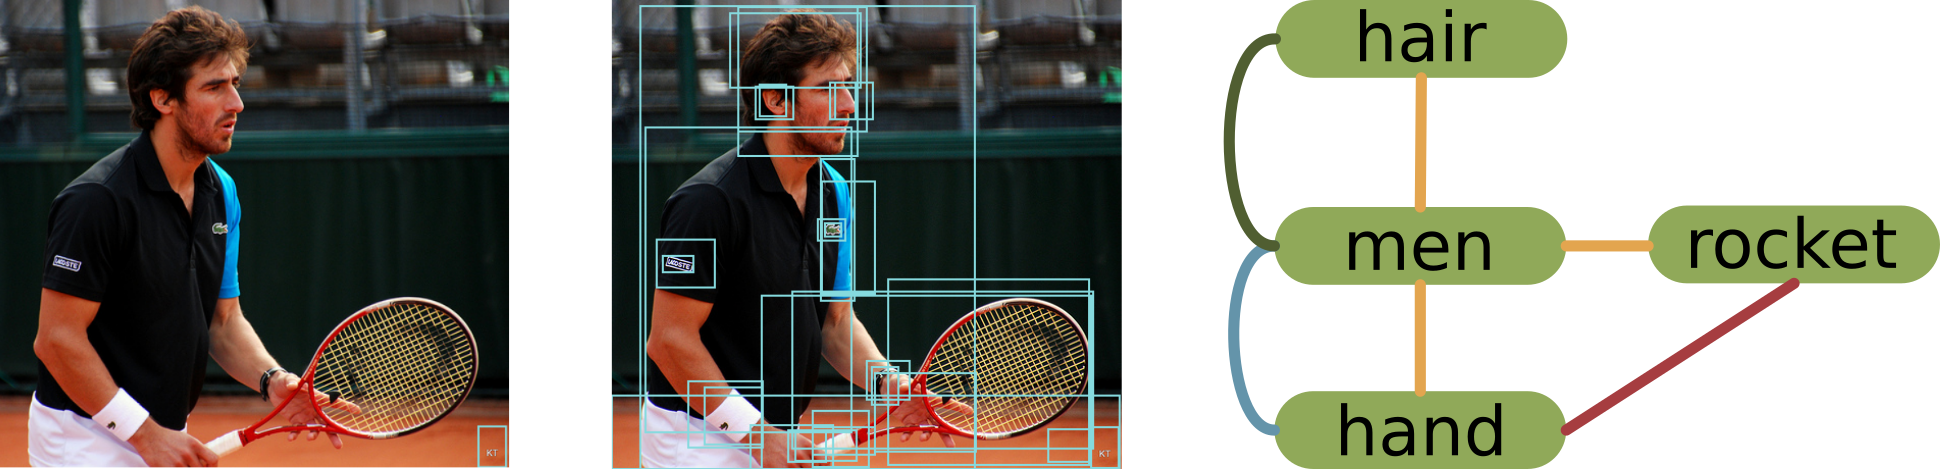
\includegraphics[width=\textwidth]{figure/scene-graph-example.png}
    \caption{Scene graph generation general view. The left part is original image, the middle part is image with detected objects and the right part is scene graph that can be obtained from such image.}
    \label{scene-graph-example}
\end{figure}

Scene graph generation is not an easy task, so let us introduce a basic scene graph generation pipeline \ref{sgg-pipeline}. It's a pity that it is not possible to use such algorithm out-of-the-box, so we will need to implement one of scene graph generation algorithms.

As an input such algorithms usually take an image with detected objects. It is not important what algorithm has been used to detect objects and regions. objects are filtered to get rid of small and redundant objects. So once we have a filtered objects it means that we have three different parts of this detection:

\begin{enumerate}
    \item Object labels and attributes.
    \item Object regions, usually in rectangle coordinate form.
    \item Convolutional features from top convolutional layer.
\end{enumerate}

Next step is to connect each object with all the others, so we have a fully-connected bipartite graph. Those connections are graph edges and they are also called relationships proposals. After that step relationships proposals are being filtered. Basically it means that algorithm compares two related objects and if they are likely not related to each other, then it will remove this relation from relations list. Then after obtaining filtered relationships we can build an unlabeled version of scene graph (with no relation labels). To label relations we apply a Graph Convolutional network, which will find a mapping of corresponding labels for each relation. It's worth to mention that the final graph is directed. If there is a relation form first object to second it doesn't mean that there is a relation from second to first.

\begin{figure}[!h]
    \centering
    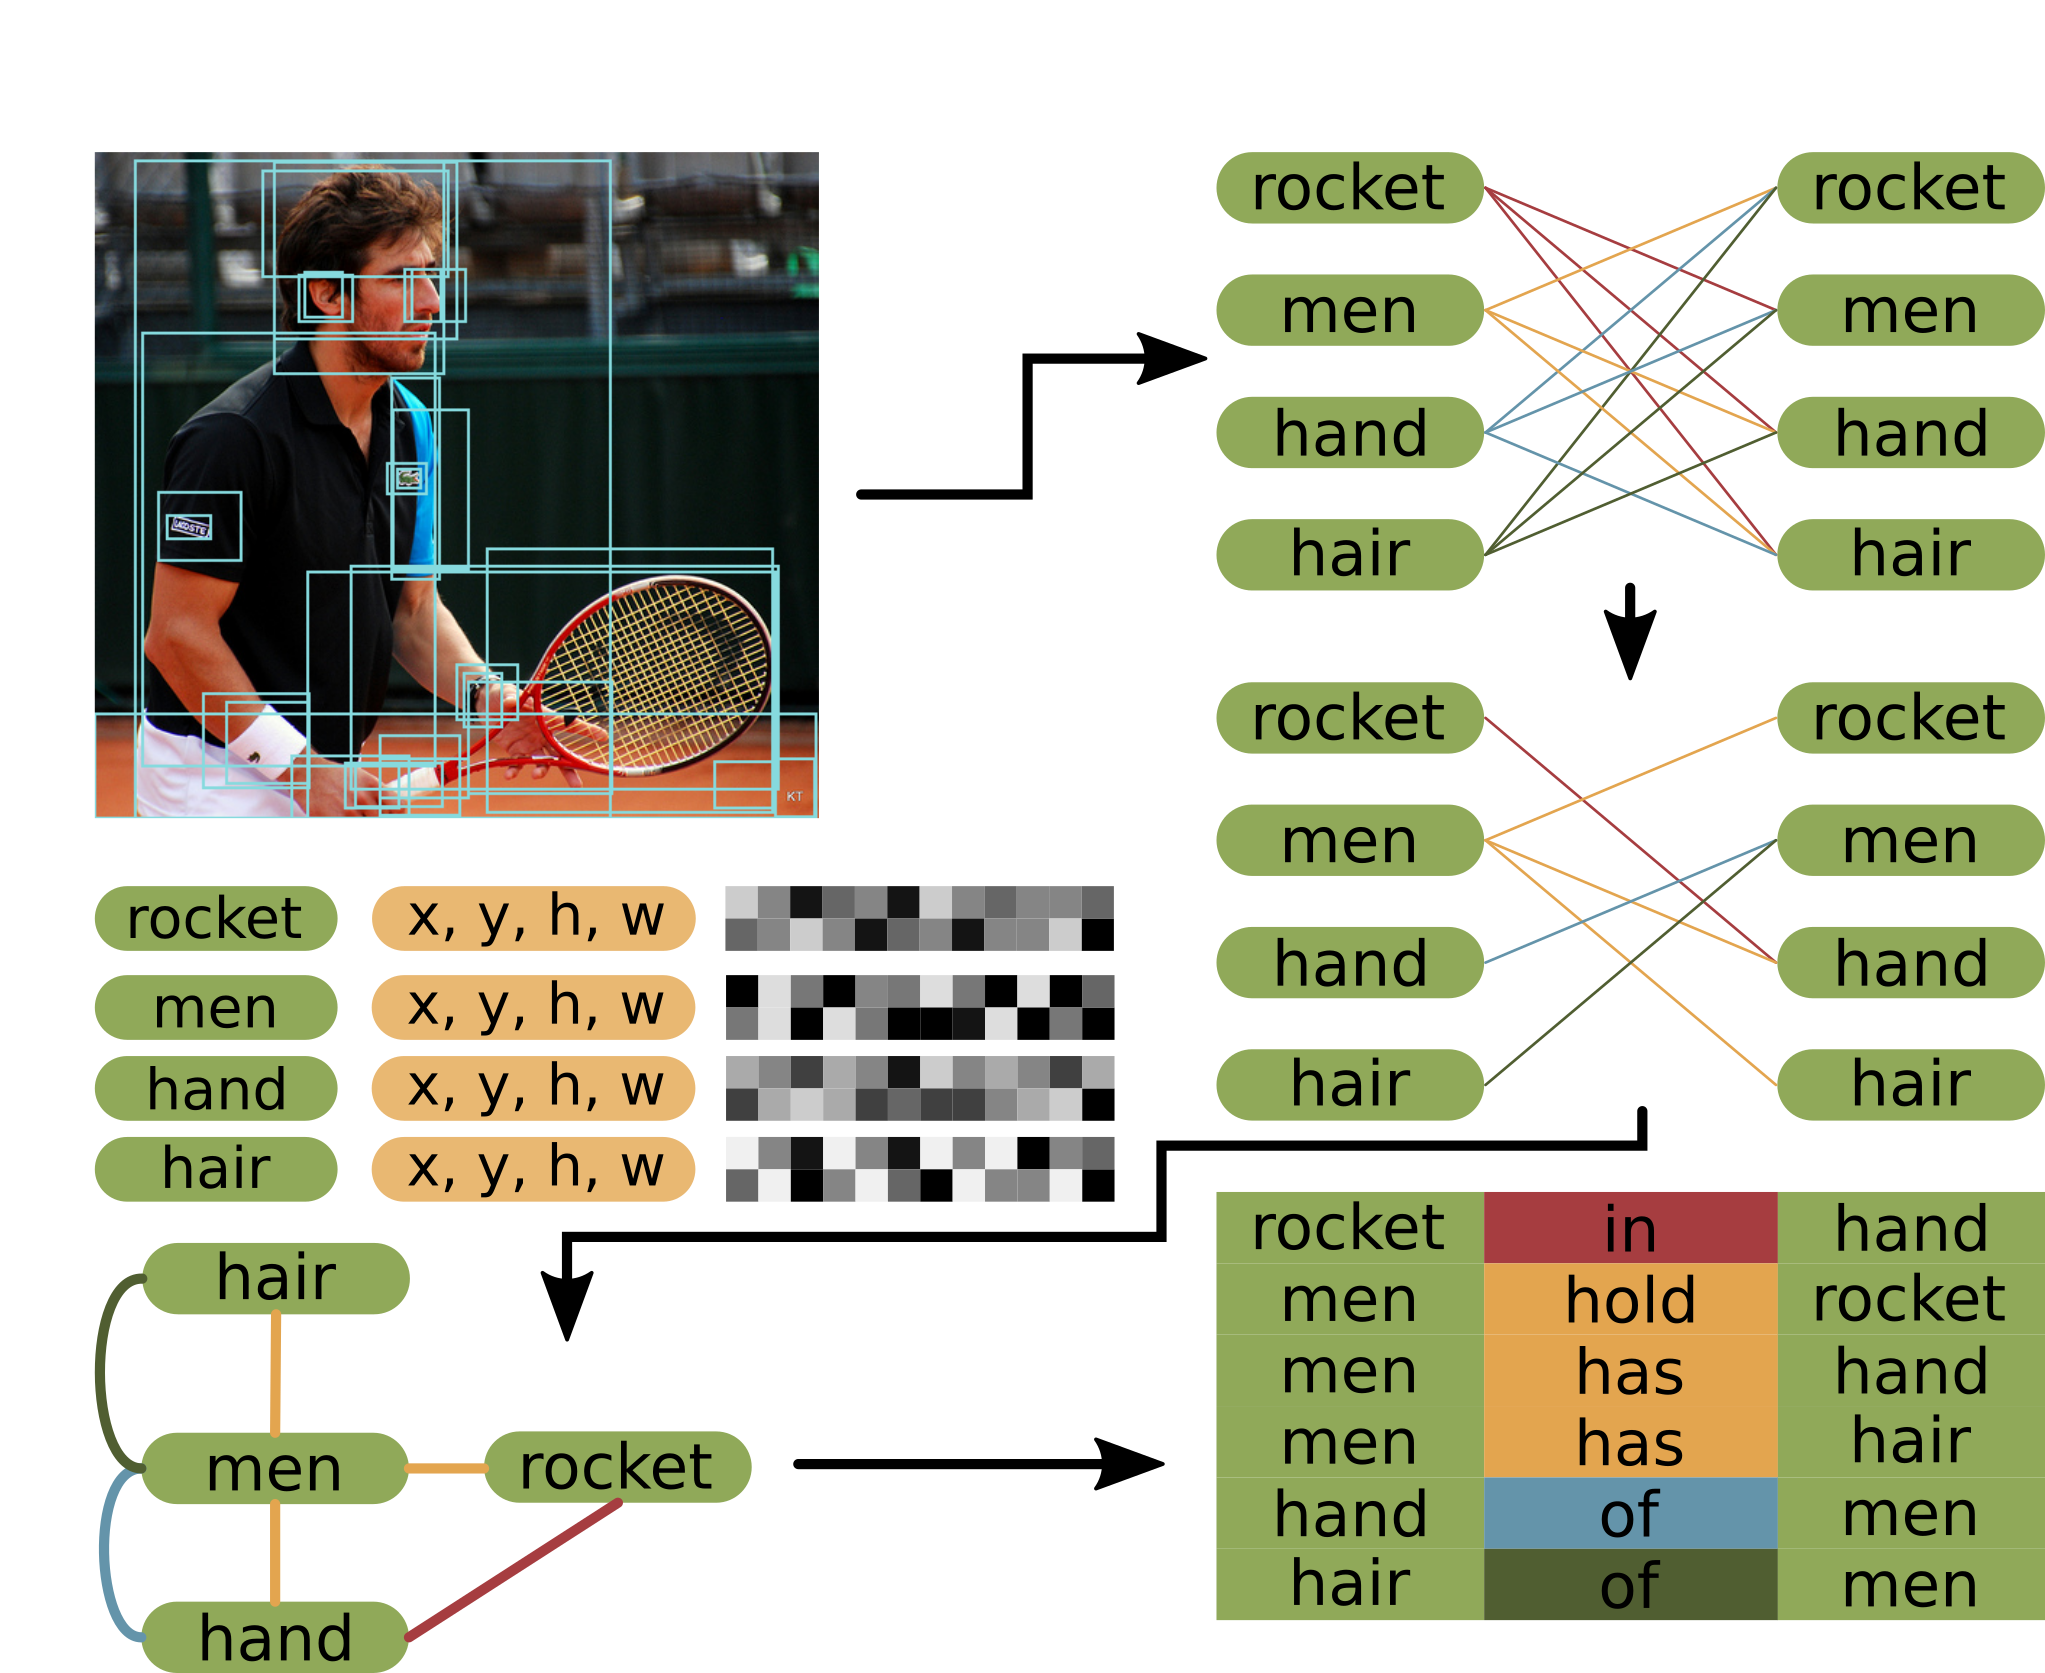
\includegraphics[width=\textwidth]{figure/sgg-pipeline.png}
    \caption{General pipeline to generate a scene graph based on objects detected from original image.}
    \label{sgg-pipeline}
\end{figure}

Having a scene graph and detected objects (objects labels and attributes, objects regions, objects convolutional features) and some convolutional feature of a scene, we can then use this information to restore an image. Figure below \ref{image-generation-from-sg} shows a general pipeline for such task.

\begin{figure}[!h]
    \centering
    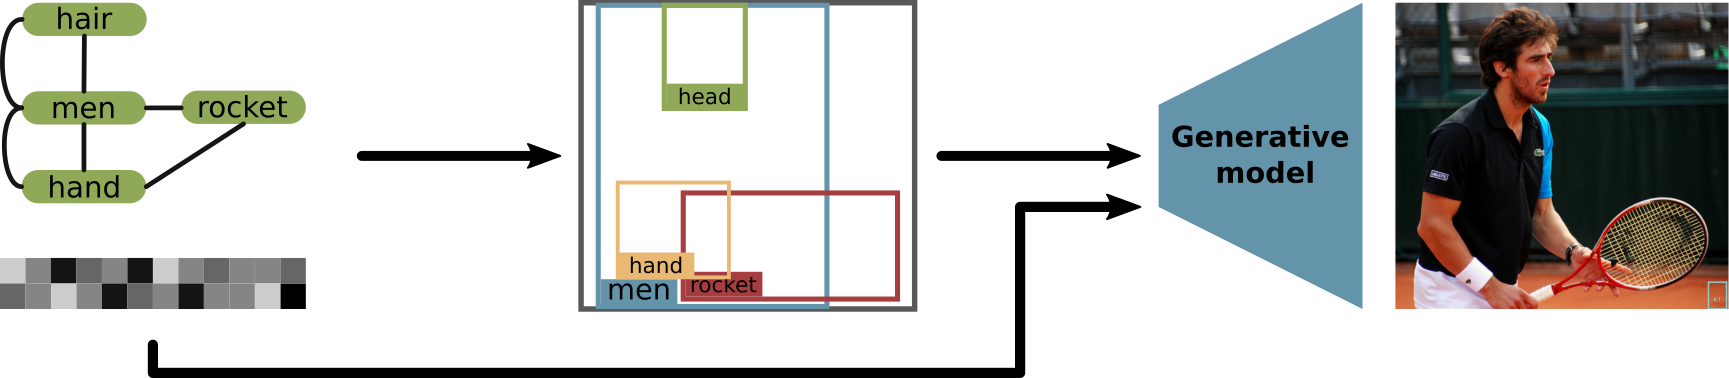
\includegraphics[width=\textwidth]{figure/image-generation-from-sg.png}
    \caption{General pipeline to generate an image from an arbitrary scene graph.}
    \label{image-generation-from-sg}
\end{figure}

As we can see from the figure, we first take a scene graph and based on objects information we build a scheme of scene, we basically map a scene to know were are the objects located and what features they have. Then such map is combined with scene convolutional features and fed in generative model, that will generate an image.

\chapter{Data}

We decided to use Visual Genome dataset, which has been used in many other works \cite{Krishna_Zhu_Groth_Johnson_Hata_Kravitz_Chen_Kalantidis_Li_Shamma_etal_2016}. Visual genome consists of more than 100,000 images labeled with scene graphs.

Dataset consists of several main parts:

\begin{enumerate}
    \item Region descriptions. Human labeled important regions of an image, each description phrase is 1 to 16 words long.
    \item Objects. Objects labeled and canonicalized to a synset ID in WordNet.
    \item Attributes. Both images and objects have attributes. They are also canonicalized to WordNet.
    \item Relationships. Connects a pair of objects. Relationships are directed.
    \item Region graphs. A graph of a region of an image. These could be more than one region graph on one image.
    \item Scene graphs. A composition of region graph of an image. One image has exactly one scene graph.
    \item Question-answer pairs. There are both region-based and freeform QA pairs.
\end{enumerate}

It might be more adequate to split the Visual Genome dataset on the following general parts for better understanding:

\begin{enumerate}
    \item Images in JPEG format with various height and width.
    \item Detected objects information (coordinates of rectangles for each object, objects labels, objects attributes).
    \item Scene graphs, obtained from images.
\end{enumerate}

The dataset itself is quite big (more then 30 Gb), so it will be required to implement a data loader that can work with such amounts of data. There were some efforts \ref{yang2018graph} to build a framework capable of working with the Visual Genome dataset, however there are no any stable version to work with.

\chapter{Schedule and arrangement}

Proposed architecture has a compound structure. As it has been mentioned above, the architecture can be separated into two major parts: encoder and decoder part. Both can be trained separately and thus implemented separately. After having first results we can already start analyzing the model performance.

It is quite a tough task to make a schedule for the following year. We decided to make it more abstract, so we can refer to this schedule as to general planing. Let us split a schedule into four quarters. For convenience reasons we organize it into table \ref{tab:schedule}.

\begin{table}
    \centering
    \caption{Schedule}
    \label{tab:schedule}
    \begin{tabular}{p{4cm}|p{8cm}|p{2cm}}
        \hline
        Task & Description & Deadline \\
        \hline
        Build a model prototype & Build a first version of a model that is capable to compress and restore images, it will include building and training encoder and decoder & September 1 \\
        \hline
        Improve model prototype & Adjust parameters, decide on additional convolutional features size & December 1 \\
        \hline
        Pack model and make it accessible for engineers & Choose an approach to pack model, implement clean and reusable library & March 1 \\
        \hline
        Write the final thesis up & Summarize research in the final thesis & June 1 \\
        \hline
    \end{tabular}
\end{table}

Tasks in this table are not really concrete. So it's more like a template for future planning. We are using Trello software to deal with concrete short-term tasks. Time management however is not a part of a technical part of the project, so we just mention it here.